\chapter{Specifikacija programske potpore}
		
	\section{Funkcionalni zahtjevi}
		
			\noindent \textbf{Dionici:}
			
			\begin{packed_enum}
				
				\item Neprijavljeni korisnici
				\item Kupci	
				\item Trgovci
				\item Administratori (nadskup razvojnog tima)
				
			\end{packed_enum}
			
			\noindent \textbf{Aktori i njihovi funkcionalni zahtjevi:}
			
			
			\begin{packed_enum}
				\item  \underbar{Neprijavljeni korisnik, tj. gost (inicijator) može:}
				
				\begin{packed_enum}
					
					\item vidjeti trgovine u blizini (TuB) kao popis
					\item prikazati TuB na karti
					\item odabrati TuB kao željenu za prikaz dostupnosti i cijena artikala
					\item vidjeti za svaki artikl s popisa posebno u kojoj je TuB najjeftiniji
					\item vidjeti za cijelu košaricu u kojoj TuB je dostupna i najjeftinija
					\item upravljati popisima
					\begin{packed_enum}
						
						\item stvarati nove popise
						\item preimenovati popise
						\item odabrati koji popis se prikazuje
						\item pretraživati artikle i dodavati ih na prikazani popis
						\item micati artikle s prikazanog popisa
						\item sve artikle s prikazanog popisa kopirati na neki drugi
						\item obrisati prikazani popis
						\item označiti artikle kao dodane u košaricu 
				
					\end{packed_enum}
					\item označiti artikl kao omiljeni za lakši pristup
					\item vidjeti mjeru pouzdanosti informacija o artiklu
					\item vidjeti ukupnu cijenu popisa
					\item vidjeti cijenu košarice
					\begin{packed_enum}
					    \item prijaviti se u sustav
					    \item registrirati se u sustav, stvoriti korisnički račun za koji su mu potrebni e-mail adresa i lozinka ili Google račun
					    \item promijeniti lozinku
					\end{packed_enum}
					
				\end{packed_enum}
				
			\item \underbar{Kupac (inicijator) može:}
				
				\begin{packed_enum}
					
					\item sve što može i neprijavljeni korisnik osim prijave
					\item glasati o ispravnosti informacija o artiklu
					\item uz skeniranje artikla napisati informacije o njemu ako su trenutne neispravne ili ih nema
					\item obrisati račun
					\item promijeniti lozinku
				\end{packed_enum}
			
			\item \underbar{Trgovac (inicijator) može:}
				
				\begin{packed_enum}
					
					\item sve što može i kupac, samo mu je za registraciju potreban dodatni verifikacijski kôd
					\item upravljati svojim trgovinama
					\begin{packed_enum}
						
						\item stvarati nove trgovine (potrebno navesti lokaciju i radno vrijeme)
						\item obrisati postojeće trgovine
						\item u bilo koju trgovinu dodati artikle s pripadnim cijenama
						\item mijenjati cijene artikala
						\item označiti da su artikli na popustu
						\item označiti da je neki artikl rasprodan
						\item maknuti artikl iz trgovine
						\item mijenjati radno vrijeme trgovine
					\end{packed_enum}
				\end{packed_enum}
			
			\item \underbar{Administrator (inicijator) može:}
				
				\begin{packed_enum}
					
					\item sve što može i kupac, samo mu je za registraciju potreban dodatni verifikacijski kôd
					\item pristupiti administratorskoj nadzornoj ploči preko web-sučelja
					\item ukloniti korisnika
					\item ukloniti trgovinu
				\end{packed_enum}
			
			
				\item \underbar{Baza podataka na poslužitelju (sudionik):}
				
				\begin{packed_enum}
					
					\item pohranjuje sve podatke o sudionicima i njihovim ovlastima
					\item pohranjuje sve podatke o artiklima
					\item pohranjuje sve podatke o trgovinama
					
				\end{packed_enum}
				
				\item \underbar{Baza podataka na uređaju (sudionik):}
				
				\begin{packed_enum}
					
					\item pohranjuje podatke o popisima i omiljenim artiklima korisnika
					
				\end{packed_enum}
				
				\item \underbar{Email poslužitelj (sudionik):}
				
				\begin{packed_enum}
					
					\item šalje privremenu lozinku korisniku koji je zaboravio svoju
					\item šalje obavijesti administratorima (o onemogućavanju pristupa jednom od njih)
					
				\end{packed_enum}
			\end{packed_enum}
			
			\eject 
			
			
				
			\subsection{Obrasci uporabe}

				\subsubsection{Opis obrazaca uporabe}
			
				
				\noindent \underbar{\textbf{UC0 - Postavljanje najveće udaljenosti}}
				\begin{packed_item}
					\item \textbf{Glavni sudionik:} Korisnik
					\item  \textbf{Cilj:} Ograničiti polumjer u kojem mogu biti rezultati pretrage trgovine
					\item  \textbf{Sudionici:} Baza podataka na poslužitelju
					\item  \textbf{Preduvjet:} Dozvoljen je pristup lokaciji
					\item  \textbf{Opis osnovnog tijeka:}
					\item[] \begin{packed_enum}
						\item Korisnik otvara postavke aplikacije
						\item Korisnik postavlja najveću udaljenost unutar koje može biti rezultat pretrage. Udaljenost se računa kao euklidska udaljenost geografske širine i dužine
						\item Ubuduće prilikom svakog upita vezanog uz trgovine osim ručne pretrage baza prvo odstrani one koje su dalje od najveće dopuštene udaljenosti od korisnika ako je pristup lokaciji još uvijek dozvoljen
					\end{packed_enum}
					\item  \textbf{Opis mogućih odstupanja:}
					\item[] \begin{packed_item}
						\item[3.a] Korisnik makne dozvolu pristupa lokaciji u nekom trenutku
						\item[] \begin{packed_enum}
							\item Ne primjenjuje se ograničenje na lokaciju trgovine 
						\end{packed_enum}
					\end{packed_item}
					\item  \textbf{Opis mogućih odstupanja:}
					\item[] \begin{packed_item}
						\item[3.b] Korisnik je na polu ili najkraći put do trgovine prelazi meridijan $\pm{180}$
						\item[] \begin{packed_enum}
							\item Korisnik potencijalno dobiva pogrešne rezultate, ali ih svi dobivaju brzo
						\end{packed_enum}
					\end{packed_item}
				\end{packed_item}
					
				%1 Stvaranje popisa
				\noindent \underbar{\textbf{UC1 - Stvaranje popisa}}
				\begin{packed_item}
					\item \textbf{Glavni sudionik:} Korisnik
					\item \textbf{Cilj:} Stvoriti novi popis artikala
					\item \textbf{Sudionici:} Baza podataka na uređaju
					\item \textbf{Preduvjet:} -
					\item \textbf{Opis osnovnog tijeka:}
					\item[] \begin{packed_enum}
						\item korisnik otvori izbornik
						\item odabere opciju "Stvori novi popis"
						\item na mjesto prikazanog popisa se stavlja novi prazni popis s pretpostavljenim imenom "Novi popis"
					\end{packed_enum}
				\end{packed_item}
				
					
				\noindent \underbar{\textbf{UC2 - Otvaranje drugog popisa}}
				\begin{packed_item}
					\item \textbf{Glavni sudionik:} Korisnik
					\item  \textbf{Cilj:} Prikazivanje određenog postojećeg popisa
					\item  \textbf{Sudionici:} Baza podataka na uređaju
					\item  \textbf{Preduvjet:} Postoji više od jednog popisa
					\item  \textbf{Opis osnovnog tijeka:}
					\item[] \begin{packed_enum}
						\item Korisnik otvori izbornik sa svim popisima
						\item Korisnik odabire popis s izbornika
						\item Drugi popis zamijenjuje prikazani
					\end{packed_enum}
					\item  \textbf{Opis mogućih odstupanja:}
					\item[] \begin{packed_item}
						\item[1.a] Nema drugih popisa
						\item[] \begin{packed_enum}
							\item Korisnik dobije obavijest da nema drugih popisa i ne otvara se izbornik
						\end{packed_enum}
					\end{packed_item}
				\end{packed_item}
				
					
				\noindent \underbar{\textbf{UC3 - Brisanje popisa}}
				\begin{packed_item}
					\item \textbf{Glavni sudionik:} Korisnik
					\item  \textbf{Cilj:} Obrisati popis
					\item  \textbf{Sudionici:} Baza podataka na uređaju
					\item  \textbf{Preduvjet:} -
					\item  \textbf{Opis osnovnog tijeka:}
					\item[] \begin{packed_enum}
						\item Korisnik otvara popis koji želi obrisati
						\item Korisnik pritisne gumb za brisanje
						\item Korisnik potvrdi da želi obrisati popis
						\item Popis se briše i prikazuje se drugi
					\end{packed_enum}
					\item  \textbf{Opis mogućih odstupanja:}
					\item[] \begin{packed_item}
						\item[4.a] Ne postoji drugi popis
						\item[] \begin{packed_enum}
							\item Stvara se novi prazni popis
						\end{packed_enum}
					\end{packed_item}
				\end{packed_item}
				
					
				\noindent \underbar{\textbf{UC4 - Preimenovanje popisa}}
				\begin{packed_item}
					\item \textbf{Glavni sudionik:} Korisnik
					\item  \textbf{Cilj:} Preimenovanje popisa
					\item  \textbf{Sudionici:} Baza podataka na uređaju
					\item  \textbf{Preduvjet:} -
					\item  \textbf{Opis osnovnog tijeka:}
					\item[] \begin{packed_enum}
						\item Korisnik dugo pritisne ime otvorenog popisa
						\item Otvori se prikaz za upis teksta
						\item Izlaskom iz prikaza se sadržaj spremi kao novo ime popisa
					\end{packed_enum}
				\end{packed_item}
			
				
				\noindent \underbar{\textbf{UC5 - Kopiranje sadržaja popisa}}
				\begin{packed_item}
					\item \textbf{Glavni sudionik:} Korisnik
					\item  \textbf{Cilj:} Sve podatke s popisa nadodati na kraj drugog popisa
					\item  \textbf{Sudionici:} Baza podataka na uređaju
					\item  \textbf{Preduvjet:} Postojanje dva popisa (predložak i odredište)
					\item  \textbf{Opis osnovnog tijeka:}
					\item[] \begin{packed_enum}
						\item Korisnik otvara popis predložak
						\item Korisnik pritisne gumb "kopiraj"
						\item Otvara se izbornik popisa
						\item Korisnik odabire popis s izbornika
						\item Svi artikli i njihove količine se dodaju na kraj popisa odredište
					\end{packed_enum}
					\item  \textbf{Opis mogućih odstupanja:}
					\item[] \begin{packed_item}
						\item[3.a] Popis odredište ne postoji
						\item[] \begin{packed_enum}
							\item Korisnik dobije obavijest da nema drugih popisa i ne otvara se izbornik
						\end{packed_enum}
					\end{packed_item}
				\end{packed_item}
				
				%6 Dodavanje artikla - Barkod
				\noindent \underbar{\textbf{UC6 - Dodavanje artikla na popis pomoću barkoda}}
					\begin{packed_item}
						\item \textbf{Glavni sudionik:} Korisnik
						\item  \textbf{Cilj:} Dodati određeni artikl na popis i u košaricu
						\item  \textbf{Sudionici:} Baza podataka na uređaju, baza podataka na poslužitelju
						\item  \textbf{Preduvjet:} Veza s poslužiteljem
						\item  \textbf{Opis osnovnog tijeka:}
						\item[] \begin{packed_enum}
							\item Korisnik pritisne gumb za dodavanje artikla na popis pomoću barkoda
							\item Korisnik skenira barkod
							\item Baza na poslužitelju vrati informacije o artiklu povezanom s barkodom
							\item Artikl se doda na kraj popisa i u košaricu, pretpostavljena količina je 1
						\end{packed_enum}
						\item  \textbf{Opis mogućih odstupanja:}
						\item[] \begin{packed_item}
							\item[2.a] Korisnik ne može pristupiti kameri, tj. barkod skeneru
							\item[] \begin{packed_enum}
								\item Sustav korisniku omogućava ručni upis znamenaka
							\end{packed_enum}
							\item[3.a] Nema informacija o artiklu u bazi podataka na poslužitelju
							\item[] \begin{packed_enum}
							    \item Upisuje se samo cijena ako postoji, inače se ispisuje poruka suosjećanja
							\end{packed_enum}
						\end{packed_item}
					\end{packed_item}
				
					
				\noindent \underbar{\textbf{UC7 - Dodavanje artikla na popis pretragom}}
				\begin{packed_item}
					\item \textbf{Glavni sudionik:} Korisnik
					\item  \textbf{Cilj:} Dodati određeni artikl na popis
					\item  \textbf{Sudionici:} Baza podataka na uređaju, baza podataka na poslužitelju
					\item  \textbf{Preduvjet:} Veza s poslužiteljem
					\item  \textbf{Opis osnovnog tijeka:}
					\item[] \begin{packed_enum}
						\item Korisnik pritisne gumb za dodavanje artikla na popis pretragom
						\item Korisnik upisuje naziv artikla
						\item Korisnik odabire jedan od ponuđenih artikala
						\item Artikl se doda na kraj popisa, pretpostavljena količina je 1
					\end{packed_enum}
					\item  \textbf{Opis mogućih odstupanja:}
					\item[] \begin{packed_item}
						\item[3.a] Nema traženog artikla
						\item[] \begin{packed_enum}
							\item Ispisuje se poruka suosjećanja na mjestu gdje bi trebali biti rezultati pretrage
						\end{packed_enum}
					\end{packed_item}
				\end{packed_item}
				
					
				\noindent \underbar{\textbf{UC8 - Dodavanje artikla na popis zadavanjem filtra}}
				\begin{packed_item}
					\item \textbf{Glavni sudionik:} Korisnik
					\item  \textbf{Cilj:} Dodati na popis artikl koji zadovoljava filter
					\item  \textbf{Sudionici:} Baza podataka na uređaju, baza podataka na poslužitelju
					\item  \textbf{Preduvjet:} Veza s poslužiteljem
					\item  \textbf{Opis osnovnog tijeka:}
					\item[] \begin{packed_enum}
						\item Korisnik pritisne gumb za dodavanje artikla na popis pomoću filtra
						\item Korisnik postavlja filter i/ili redukciju (min, max)
						\item Artikl koji zadovoljava filter se doda na kraj popisa, pretpostavljena količina je 1
					\end{packed_enum}
					\item  \textbf{Opis mogućih odstupanja:}
					\item[] \begin{packed_item}
						\item[3.a] Više artikala zadovoljava filtar i/ili redukciju
						\item[] \begin{packed_enum}
							\item Odabire se onaj s najnižom cijenom koji je najbliži ako je dozvoljen pristup lokaciji, inače prvi u bazinom odgovoru na upit
						\end{packed_enum}
					\end{packed_item}
				\end{packed_item}
				
					
				\noindent \underbar{\textbf{UC9 - Dodavanje artikla iz popisa omiljenih artikala}}
				\begin{packed_item}
					\item \textbf{Glavni sudionik:} Korisnik
					\item  \textbf{Cilj:} Dodati na popis artikl iz popisa omiljenih artikala
					\item  \textbf{Sudionici:} Baza podataka na uređaju
					\item  \textbf{Preduvjet:} Postoji omiljeni artikl
					\item  \textbf{Opis osnovnog tijeka:}
					\item[] \begin{packed_enum}
						\item Korisnik otvori bočnu traku
						\item Korisnik pritisne željeni artikl
						\item Artikl se doda na kraj popisa, pretpostavljena količina je 1
						\item Popis se osvježi
					\end{packed_enum}
				\end{packed_item}
			
				
				\noindent \underbar{\textbf{UC10 - Zamjena artikla na popisu nekim drugim artiklom}}
				\begin{packed_item}
					\item \textbf{Glavni sudionik:} Korisnik
					\item  \textbf{Cilj:} Zamijeniti artikl na popisu nekim drugim artiklom
					\item  \textbf{Sudionici:} Baza podataka na uređaju, baza podataka na poslužitelju
					\item  \textbf{Preduvjet:} Postoji artikl na popisu, veza s poslužiteljem
					\item  \textbf{Opis osnovnog tijeka:}
					\item[] \begin{packed_enum}
						\item Korisnik povuče artikl na popisu ulijevo
						\item Korisnik odabire novi artikl na onaj način na koji je dodan stari artikl
						\item Novi artikl je prikazan na mjestu starog, pretpostavljena količina je 1
					\end{packed_enum}
				\end{packed_item}
			
				
				\noindent \underbar{\textbf{UC11 - Micanje artikla s popisa}}
				\begin{packed_item}
					\item \textbf{Glavni sudionik:} Korisnik
					\item  \textbf{Cilj:} U potpunosti maknuti artikl s popisa
					\item  \textbf{Sudionici:} Baza podataka na uređaju
					\item  \textbf{Preduvjet:} Postoji artikl na popisu
					\item  \textbf{Opis osnovnog tijeka:}
					\item[] \begin{packed_enum}
						\item Korisnik povuče artikl na popisu udesno
						\item Artikl se miče s popisa
					\end{packed_enum}
				\end{packed_item}
			
				
				\noindent \underbar{\textbf{UC12 - Registracija korisnika}}
				\begin{packed_item}
					\item \textbf{Glavni sudionik:} Gost
					\item  \textbf{Cilj:} Stvaranje korisničkog računa
					\item  \textbf{Sudionici:} Baza podataka na poslužitelju
					\item  \textbf{Preduvjet:} Veza s poslužiteljem
					\item  \textbf{Opis osnovnog tijeka:}
					\item[] \begin{packed_enum}
						\item Gost otvara izbornik
						\item Gost u izborniku odabire "Registracija"
						\item Gost upisuje email, lozinku i potvrdu lozinke za registraciju kao kupac. Dodatno tajni broj za registraciju kao trgovac ili administrator
						\item Baza provjerava postoji li već korisnik s istom adresom elektroničke pošte
						\item Korisnik dobiva povratnu informaciju
					\end{packed_enum}
					\item  \textbf{Opis mogućih odstupanja:}
					\item[] \begin{packed_item}
						\item[3.a] Email adresa je u neispravnom obliku, lozinka ima manje od 8 znakova ili se potvrda ne podudara
						\item[] \begin{packed_enum}
							\item Korisnik dobiva odgovarajuću informativnu poruku, podatci se ne brišu ni ne šalju
						\end{packed_enum}
						\item[4.a] U bazi već postoji korisnikova mail adresa
						\item[] \begin{packed_enum}
							\item Korisnik dobiva odgovarajuću informativnu poruku, podatci se ne brišu
						\end{packed_enum}
					\end{packed_item}
				\end{packed_item}
			
				
				\noindent \underbar{\textbf{UC13 - Prijava korisnika}}
				\begin{packed_item}
					\item \textbf{Glavni sudionik:} Gost
					\item  \textbf{Cilj:} Prijava u sustav
					\item  \textbf{Sudionici:} Baza podataka na poslužitelju, email poslužitelj u slučaju odstupanja 2.a
					\item  \textbf{Preduvjet:} Veza s poslužiteljima (sustav, baza podataka i email), gost ima račun
					\item  \textbf{Opis osnovnog tijeka:}
					\item[] \begin{packed_enum}
						\item Gost otvara sučelje za prijavu
						\item Gost upisuje email adresu i lozinku ili se prijavi pomoću Google računa
						\item Baza podataka provjerava dane informacije
						\item Gost dobije povratnu informaciju
					\end{packed_enum}
					\item  \textbf{Opis mogućih odstupanja:}
					\item[] \begin{packed_item}
						\item[2.a] Korisnik ne zna koju lozinku ima ili više ne želi koristiti postojeću
						\item[] \begin{packed_enum}
							\item Korisnik pritisne gumb "Promijeni lozinku"
							\item Korisnik upiše svoju mail adresu
							\item Sustav preko email poslužitelja šalje poruku s privremenom lozinkom koju sprema u bazu
							\item Korisnik dobiva novu lozinku na mail adresu
							\item Korisnik se prijavi u aplikaciju i promijeni lozinku (UC15)
						\end{packed_enum}
					    \item[3.a] Email adresa je u neispravnom obliku ili lozinka ima manje od 8 znakova
						\item[] \begin{packed_enum}
							\item Korisnik dobiva odgovarajuću informativnu poruku, podatci se ne brišu ni ne šalju
						\end{packed_enum}
						\item[3.b] U bazi ne postoji korisnikova mail adresa s pripadnom lozinkom ili je račun označen kao onemogućen
						\item[] \begin{packed_enum}
							\item Korisnik dobiva odgovarajuću informativnu poruku
						\end{packed_enum}
					\end{packed_item}
				\end{packed_item}
			
				
				\noindent \underbar{\textbf{UC14 - Odjava korisnika}}
				\begin{packed_item}
					\item \textbf{Glavni sudionik:} Prijavljeni korisnik (kupac, trgovac ili administrator)
					\item  \textbf{Cilj:} Prijeći u način rada neprijavljenog korisnika
					\item  \textbf{Sudionici:} Baza podataka na poslužitelju
					\item  \textbf{Preduvjet:} Veza s poslužiteljem, korisnik je prijavljen
					\item  \textbf{Opis osnovnog tijeka:}
					\item[] \begin{packed_enum}
						\item Prijavljeni korisnik otvara izbornik
						\item Prijavljeni korisnik u izborniku odabire "Odjava"
						\item Korisnik je odjavljen
					\end{packed_enum}
				\end{packed_item}
				
			
				
				\noindent \underbar{\textbf{UC15 - Promjena lozinke}}
				\begin{packed_item}
					\item \textbf{Glavni sudionik:} Prijavljeni korisnik
					\item  \textbf{Cilj:} Promijeniti lozinku 
					\item  \textbf{Sudionici:} Baza podataka na poslužitelju
					\item  \textbf{Preduvjet:} Veza s poslužiteljem, korisnik je prijavljen email adresom i lozinkom
					\item  \textbf{Opis osnovnog tijeka:}
					\item[] \begin{packed_enum}
						\item Prijavljeni korisnik otvara izbornik
						\item Prijavljeni korisnik u izborniku odabire "Promjena lozinke"
						\item Prijavljeni korisnik upiše staru lozinku, novu lozinku i potvrdu nove lozinke
						\item Prijavljeni korisnik dobiva obavijest o uspješnoj promjeni lozinke
					\end{packed_enum}
					\item  \textbf{Opis mogućih odstupanja:}
					\item[] \begin{packed_item}
						\item[3.a] Korisnikova trenutna lozinka nije ispravna ili se potvrda nove lozinke ne podudara
						\item[] \begin{packed_enum}
							\item Korisnik dobiva odgovarajuću informativnu poruku
						\end{packed_enum}
					\end{packed_item}
				\end{packed_item}
			
				
				\noindent \underbar{\textbf{UC16 - Pregled informacija o artiklu}}
				\begin{packed_item}
					\item \textbf{Glavni sudionik:} Korisnik
					\item  \textbf{Cilj:} Pregledati informacije o artiklu
					\item  \textbf{Sudionici:} Baza podataka na poslužitelju
					\item  \textbf{Preduvjet:} Veza s poslužiteljem i artikl na popisu
					\item  \textbf{Opis osnovnog tijeka:}
					\item[] \begin{packed_enum}
						\item Korisnik pritisne ime ili cijenu artikla na popisu
						\item Korisniku se prikažu informacije o artiklu i mjera pouzdanosti tih informacija
					\end{packed_enum}
				\end{packed_item}
			
				
				\noindent \underbar{\textbf{UC17 - Izmjena informacija o artiklu}}
				\begin{packed_item}
					\item \textbf{Glavni sudionik:} Prijavljeni korisnik
					\item  \textbf{Cilj:} Pregledati i izmijeniti informacije o artiklu
					\item  \textbf{Sudionici:} Baza podataka na poslužitelju
					\item  \textbf{Preduvjet:} Korisnik treba biti prijavljen, imati vezu s poslužiteljem i artikl na popisu
					\item  \textbf{Opis osnovnog tijeka:}
					\item[] \begin{packed_enum}
						\item Korisnik pregleda informacije o artiklu
						\item Prijavljeni korisnik glasa o ispravnosti informacija
						\item Nakon davanja negativnog glasa, prijavljeni korisnik može odabrati drugi opis ili uređuje postojeći
						\item Prijavljeni korisnik skenira barkod tog proizvoda
						\item Promjena se spremi u bazu podataka
						\item Prijavljeni korisnik ubuduće vidi onaj opis koji je odabrao ili napisao te se tom opisu broj glasova poveća za jedan
					\end{packed_enum}
				\end{packed_item}
			
				
				\noindent \underbar{\textbf{UC18 - Omiljeni proizvodi}}
				\begin{packed_item}
					\item \textbf{Glavni sudionik:} Korisnik
					\item  \textbf{Cilj:} Učiniti artikl lakše dostupnim za dodavanje na popis, poništiti tu akciju
					\item  \textbf{Sudionici:} Baza podataka na uređaju
					\item  \textbf{Preduvjet:} Artikl je na popisu
					\item  \textbf{Opis osnovnog tijeka:}
					\item[] \begin{packed_enum}
						\item Korsinik otvori informacije o  artiklu
						\item Korisnik pritisne na zvjezdicu
						\item Ako artikl nije na popisu omiljenih proizvoda, pojavit će se na njemu, u suprotnom će se maknuti s njega
						\item Za pregled omiljenih proizvoda korisnik otvara bočnu traku
					\end{packed_enum}
				\end{packed_item}
			
				
				\noindent \underbar{\textbf{UC19 - Najjeftinija trgovina}}
				\begin{packed_item}
					\item \textbf{Glavni sudionik:} Korisnik
					\item  \textbf{Cilj:} Prikazati trgovinu u kojoj je zbroj cijena zadanih artikala najniža
					\item  \textbf{Sudionici:} Baza podataka na poslužitelju, baza podataka na uređaju
					\item  \textbf{Preduvjet:} Veza s poslužiteljem
					\item  \textbf{Opis osnovnog tijeka:}
					\item[] \begin{packed_enum}
						\item Korisnik otvara izbornik načina izračna cijena
						\item U izborniku bira "Najjeftinija trgovina"
						\item Cijene se osvježe
						\item Ponovno osvježavanje popisa korisnik pokreće povlačenjem popisa prema dolje, pritom se porast cijene označava promjenom njene boje u crvenu, a pad u zelenu (UC18.1)
						\item Za informacije o trgovini korisnik pritisne na cijenu artikla
					\end{packed_enum}
					\item  \textbf{Opis mogućih odstupanja:}
					\item[] \begin{packed_item}
						\item[3.a] Ne postoji trgovina sa svim artiklima s popisa
						\item[] \begin{packed_enum}
							\item Bira se trgovina koja ima najviše artikala na popisu, ako ima više takvih onda ona s najviše artikala općenito, a ako takvih ima više, onda ona koja bude prva u bazinom odgovoru na upit. Artiklima kojih nema u trgovini se zacrveni oznaka količine.
						\end{packed_enum}
						\item[3.b] Postoji više trgovina s najnižom cijenom popisa
						\item[] \begin{packed_enum}
							\item Odabire se najbliža ako je dozvoljen pristup lokaciji, inače prva u bazinom odgovoru na upit
						\end{packed_enum}
						\item[4.a] Cijena cijelog popisa postane manja u drugoj trgovini ili neki artikli postanu nedostupni u trenutnoj trgovini ili cijela trgovina postane nedostupna
						\item[] \begin{packed_enum}
							\item Trenutna trgovina se promijeni u onu koja ima sve artikle i najnižu cijenu popisa
						\end{packed_enum}
						\item[4.b] Artikl ne postoji više niti u jednoj trgovini
						\item[] \begin{packed_enum}
							\item Naziv artikla promijeni boju u crvenu
						\end{packed_enum}
					\end{packed_item}
				\end{packed_item}
			
				
				\noindent \underbar{\textbf{UC20 - Najjeftiniji artikli}}
				\begin{packed_item}
					\item \textbf{Glavni sudionik:} Korisnik
					\item  \textbf{Cilj:} Prikazati za svaki artikl najnižu cijenu
					\item  \textbf{Sudionici:} Baza podataka na uređaju, baza podataka na poslužitelju
					\item  \textbf{Preduvjet:} Veza s poslužiteljem
					\item  \textbf{Opis osnovnog tijeka:}
					\item[] \begin{packed_enum}
						\item Korisnik otvara izbornik načina izračuna cijena
						\item U izborniku bira "Najjeftiniji artikli"
						\item Cijene se osvježe
						\item Ponovno osvježavanje popisa korisnik pokreće povlačenjem popisa prema dolje, pritom se porast cijene označava promjenom njene boje u crvenu, a pad u zelenu (19.1)
						\item Za informacije o trgovini u kojoj je cijena dostupna korisnik pritisne na cijenu artikla
					\end{packed_enum}
					\item  \textbf{Opis mogućih odstupanja:}
					\item[] \begin{packed_item}
						\item[3.a] Postoji više trgovina s najnižom cijenom artikla
						\item[] \begin{packed_enum}
							\item Odabire se najbliža ako je dozvoljen pristup lokaciji, inače prva u bazinom odgovoru na upit
						\end{packed_enum}
						\item[4.a] Artikl s popisa više nije u ponudi u trenutnoj trgovini, skuplji je nego negdje drugo ili trenutna trgovina više ne postoji
						\item[] \begin{packed_enum}
							\item Cijena se uzme iz trgovine gdje je najjeftinija
						\end{packed_enum}
						\item[4.b] Artikl ne postoji više niti u jednoj trgovini
						\item[] \begin{packed_enum}
							\item Naziv artikla promijeni boju u crvenu
						\end{packed_enum}
					\end{packed_item}
				\end{packed_item}
			
				
				\noindent \underbar{\textbf{UC21 - Prikaz cijena u točno određenoj trgovini}}
				\begin{packed_item}
					\item \textbf{Glavni sudionik:} Korisnik
					\item  \textbf{Cilj:} Prikazati cijene artikala u točno određenoj košarici
					\item  \textbf{Sudionici:} Baza podataka na uređaju, baza podataka na poslužitelju
					\item  \textbf{Preduvjet:} Veza s poslužiteljem
					\item  \textbf{Opis osnovnog tijeka:}
					\item[] \begin{packed_enum}
						\item Korisnik otvara izbornik načina izračuna cijena
						\item U izborniku bira "Određena trgovina"
						\item Korisnik upisuje naziv trgovine
						\item Korisnik odabire jednu od ponuđenih trgovina. Ako je dozvoljen pristup lokaciji, poredane su po udaljenosti od korisnika
						\item Cijene se osvježe Pipijem
						\item Ponovno osvježavanje popisa korisnik pokreće povlačenjem popisa prema dolje
						\item Za informacije o trgovini korisnik pritisne na cijenu artikla
					\end{packed_enum}
					\item  \textbf{Opis mogućih odstupanja:}
					\item[] \begin{packed_item}
						\item[4.a] Nema tražene trgovine
						\item[] \begin{packed_enum}
							\item Ispisuje se poruka suosjećanja na mjestu gdje bi trebali biti rezultati pretrage
						\end{packed_enum}
						\item[5.a] Nema artikla s popisa u zadanoj trgovini
						\item[] \begin{packed_enum}
							\item Artiklu se oznaka količine zacrveni označavajući da ga nema u skladištu
						\end{packed_enum}
						\item[6.a] Artikl s popisa više nije u ponudi u zadanoj trgovini
						\item[] \begin{packed_enum}
							\item Oznaka količine artikla promijeni boju u crvenu
						\end{packed_enum}
						\item[6.b] Artikl ne postoji više niti u jednoj trgovini i/ili trgovina više ne postoji
						\item[] \begin{packed_enum}
							\item Naziv artikla i/ili trgovine promijeni boju u crvenu
						\end{packed_enum}
					\end{packed_item}
				\end{packed_item}
			
				
				\noindent \underbar{\textbf{UC22 - Dodavanje trgovine}}
				\begin{packed_item}
					\item \textbf{Glavni sudionik:} Trgovac
					\item  \textbf{Cilj:} Dodati informacije o trgovini
					\item  \textbf{Sudionici:} Baza podataka na poslužitelju
					\item  \textbf{Preduvjet:} Trgovac je prijavljen u sustav
					\item  \textbf{Opis osnovnog tijeka:}
					\item[] \begin{packed_enum}
						\item Trgovac otvara svoju nadzornu ploču
						\item Trgovac odabire opciju "Dodaj trgovinu"
						\item Za dodavanje trgovine trgovac upisuje naziv trgovine, njenu adresu, radno vrijeme i koordinate
					\end{packed_enum}
				\end{packed_item}
			
				
				\noindent \underbar{\textbf{UC23 - Brisanje trgovine}}
				\begin{packed_item}
					\item \textbf{Glavni sudionik:} Trgovac ili administrator
					\item  \textbf{Cilj:} Obrisati trgovinu iz sustava
					\item  \textbf{Sudionici:} Baza podataka na poslužitelju
					\item  \textbf{Preduvjet:} Trgovac je prijavljen u sustav
					\item  \textbf{Opis osnovnog tijeka:}
					\item[] \begin{packed_enum}
						\item Trgovac ili administrator otvara svoju nadzornu ploču
						\item Trgovac ili administrator odabire trgovinu koju ju želi obrisati
						\item Trgovac ili administrator pritisne gumb za brisanje i potvrdi odluku
						\item Baza obriše podatke o trgovini
						\item Trgovac dobiva potvrdu na mail o brisanju trgovine
					\end{packed_enum}
				\end{packed_item}
			
				
				\noindent \underbar{\textbf{UC24 -  Mijenjanje podataka o trgovini}}
				\begin{packed_item}
					\item \textbf{Glavni sudionik:} Trgovac
					\item  \textbf{Cilj:} Promijeniti podatke o trgovini ili artiklima u njima
					\item  \textbf{Sudionici:} Baza podataka na poslužitelju
					\item  \textbf{Preduvjet:} Trgovac je prijavljen u sustav
					\item  \textbf{Opis osnovnog tijeka:}
					\item[] \begin{packed_enum}
						\item Trgovac otvara svoju nadzornu ploču
						\item Trgovac odabire trgovinu kojoj želi promijeniti podatke
						\item Trgovac promijeni željene podatke ili doda nove artikle kao petorku (barkod, cijena, popust, dostupnost, email\_zeljenog\_opisivaca) ili ih doda više odjednom kao csv datoteku
						\item Baza podataka spremi promjene
					\end{packed_enum}
					\item  \textbf{Opis mogućih odstupanja:}
					\item[] \begin{packed_item}
						\item[3.a] Informacije o artiklima ne odgovaraju zadanom formatu
						\item[] \begin{packed_enum}
							\item Akcija ili transakcija se prekida i trgovac dobiva odgovarajuću informativnu poruku
						\end{packed_enum}
						\item[3.b] Polje "email\_zeljenog\_opisivaca" je "None" ili mail nekoga tko nije opisao dani artikl
						\item[] \begin{packed_enum}
							\item S trgovinom neće biti povezan određeni opis artikla nego će se prikazivati pretpostavljeni (onaj s najviše pozitivnih glasova)
						\end{packed_enum}
					\end{packed_item}
				\end{packed_item}
			
				
				\noindent \underbar{\textbf{UC25 - Onemogućenje pristupa}}
				\begin{packed_item}
					\item \textbf{Glavni sudionik:} Administrator
					\item  \textbf{Cilj:} Onemogućavanje pristupa kupcu
					\item  \textbf{Sudionici:} Baza podataka na poslužitelju, email poslužitelj u slučaju odstupanja 3.a
					\item  \textbf{Preduvjet:} Administrator je prijavljen u sustav na web sučelju, veza s poslužiteljima (email, baza podataka i sustav)
					\item  \textbf{Opis osnovnog tijeka:}
					\item[] \begin{packed_enum}
						\item Administrator otvara svoju nadzornu ploču na web-sučelju
						\item Administrator odabire opciju "Zabrani pristup korisničkom računu"
						\item Administrator odabire račun kojem želi zabraniti pristup
						\item Baza podataka označava račun kao onemogućen
						\item Korisnik je odjavljen čim uspostavi vezu s poslužiteljem
					\end{packed_enum}
					\item  \textbf{Opis mogućih odstupanja:}
					\item[] \begin{packed_item}
						\item[3.a] Odabran je administratorski račun
						\item[] \begin{packed_enum}
							\item Račun je označen jednom, ali ne gubi funkcionalnost dok ga ne označi bar 50\% administratora u istom danu
							\item Šalje se email poruka svim ostalim administratorima tko koga pokušava onemogućiti 
						\end{packed_enum}
					\end{packed_item}
				\end{packed_item}
			
				
				\noindent \underbar{\textbf{UC26 - Uklanjanje opisa artikla}}
				\begin{packed_item}
					\item \textbf{Glavni sudionik:} Administrator
					\item  \textbf{Cilj:} Uklanjanje opisa artikla iz sustava
					\item  \textbf{Sudionici:} Baza podataka na poslužitelju
					\item  \textbf{Preduvjet:} Administrator je prijavljen u sustav
					\item  \textbf{Opis osnovnog tijeka:}
					\item[] \begin{packed_enum}
						\item Administrator otvara svoju nadzornu ploču na web-sučelju
						\item Administrator odabire opciju "Uredi artikle"
						\item Administrator odabire opis artikla koji želi maknuti
						\item Administrator vidi mail adresu koorisnika koji je napisao sporni opis
						\item Administrator pritisne gumb "Ukloni opis artikla"
						\item Baza uklanja opis artikla
					\end{packed_enum}
				\end{packed_item}
			
				
				\noindent \underbar{\textbf{UC27 - Dodavanje tajnog broja za registraciju}}
				\begin{packed_item}
					\item \textbf{Glavni sudionik:} Administrator
					\item  \textbf{Cilj:} Omogućiti registraciju trgovcu i/ili administratoru
					\item  \textbf{Sudionici:} Baza podataka na poslužitelju
					\item  \textbf{Preduvjet:} Administrator je prijavljen u sustav
					\item  \textbf{Opis osnovnog tijeka:}
					\item[] \begin{packed_enum}
						\item Administrator otvara svoju nadzornu ploču na web-sučelju
						\item Administrator odabire opciju "Dodaj verifikaciju"
						\item Administrator dodaje tajni broj i email za registraciju
						\item Podatci se spremaju u bazu podataka
					\end{packed_enum}
				\end{packed_item}
				\eject
					
			\subsubsection{Dijagrami obrazaca uporabe}
			    \begin{figure}[H]
			        \begin{center}
		            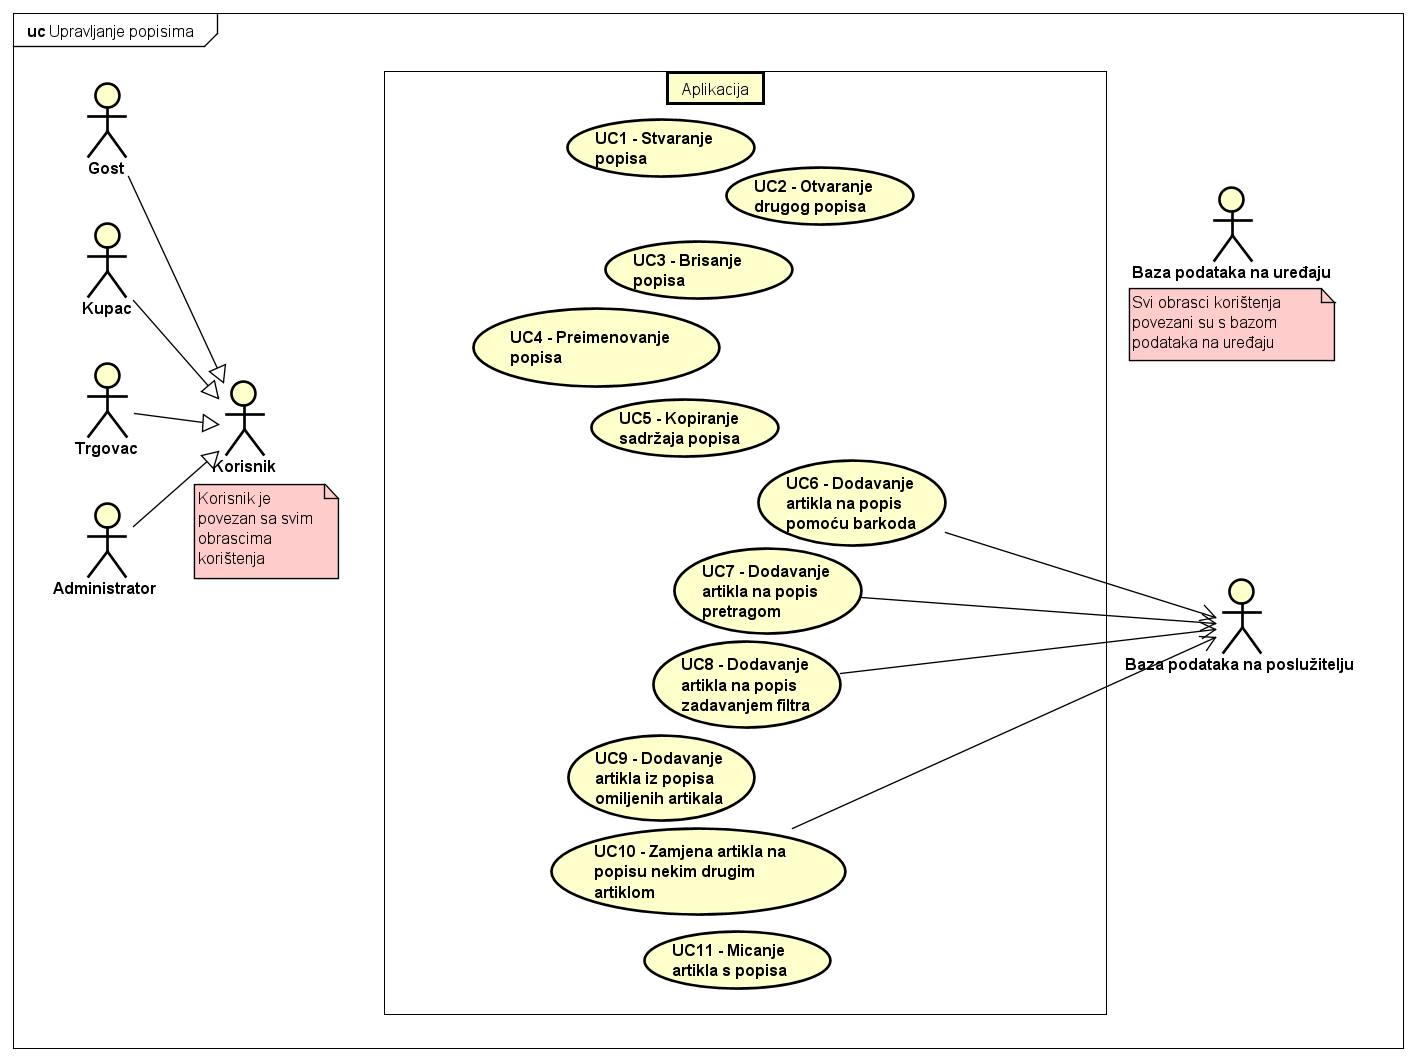
\includegraphics[width=.9\linewidth]{dijagrami/uc_upravljanje_popisima.png}
		            \label{fig:uc_upravljanje_popisima}
	                \end{center}
	            \end{figure}		
			    \begin{figure}[H]
			        \begin{center}
		            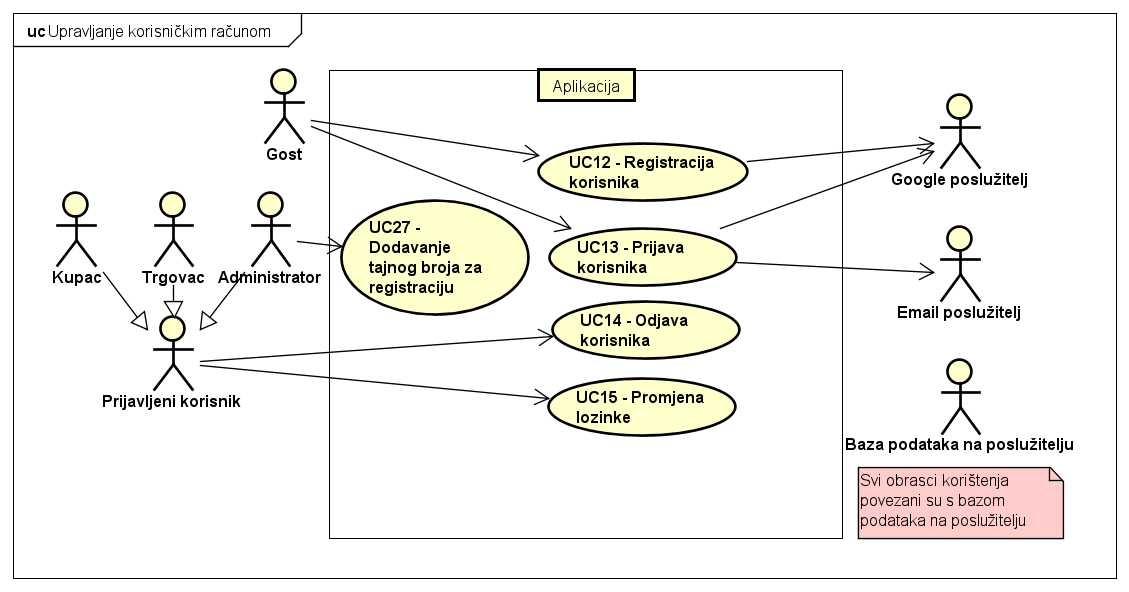
\includegraphics[width=.9\linewidth]{dijagrami/uc_kor_racun.png}
		            \label{fig:uc_kor_racun}
	                \end{center}
	            \end{figure}		
			    \begin{figure}[H]
			        \begin{center}
		            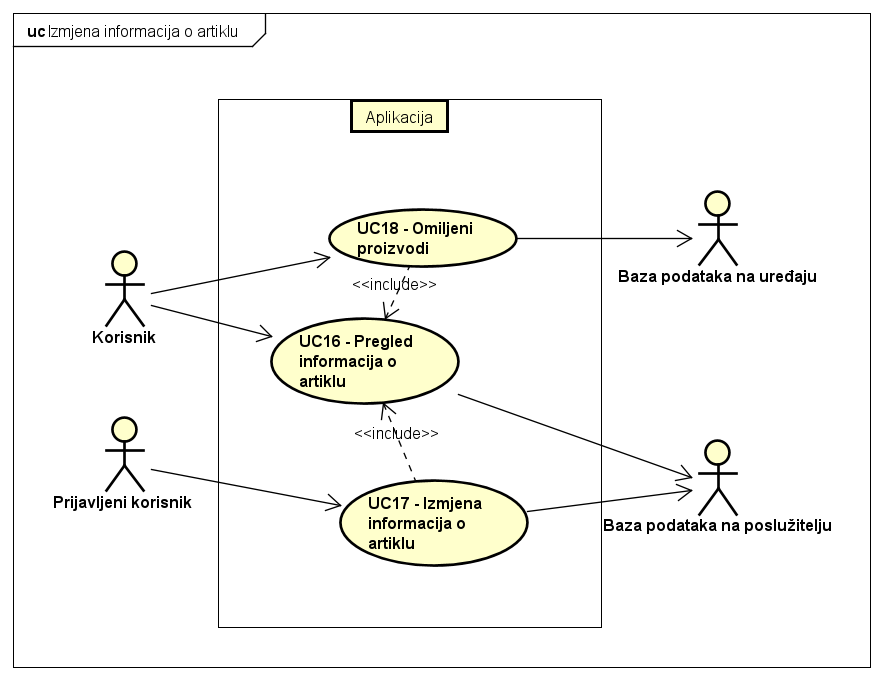
\includegraphics[width=.9\linewidth]{dijagrami/uc_info_artikl.png}
		            \label{fig:uc_info_artikl}
	                \end{center}
	            \end{figure}		
			    \begin{figure}[H]
			        \begin{center}
		            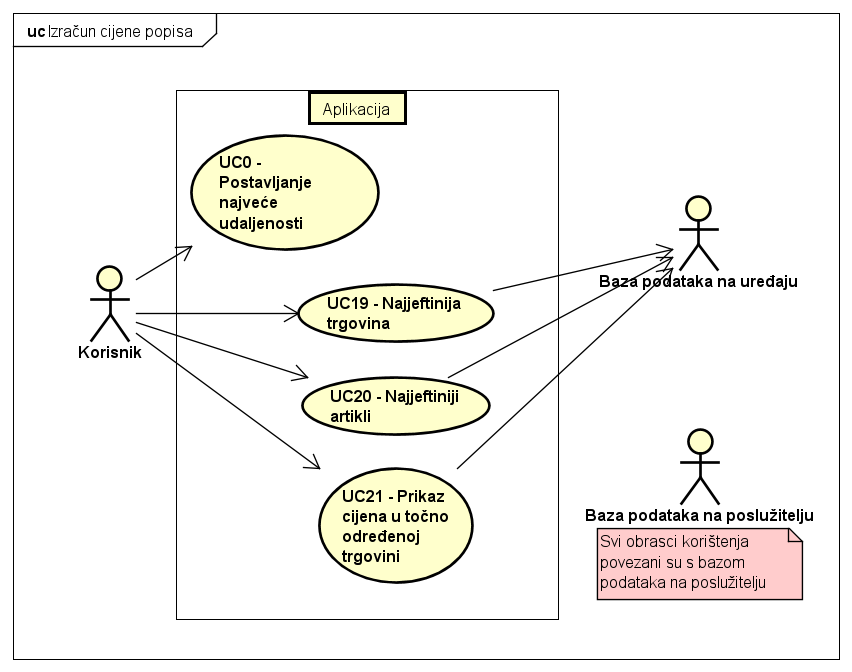
\includegraphics[width=.9\linewidth]{dijagrami/uc_cijena_popisa.png}
		            \label{fig:uc_cijena_popisa}
	                \end{center}
	            \end{figure}		
			    \begin{figure}[H]
			        \begin{center}
		            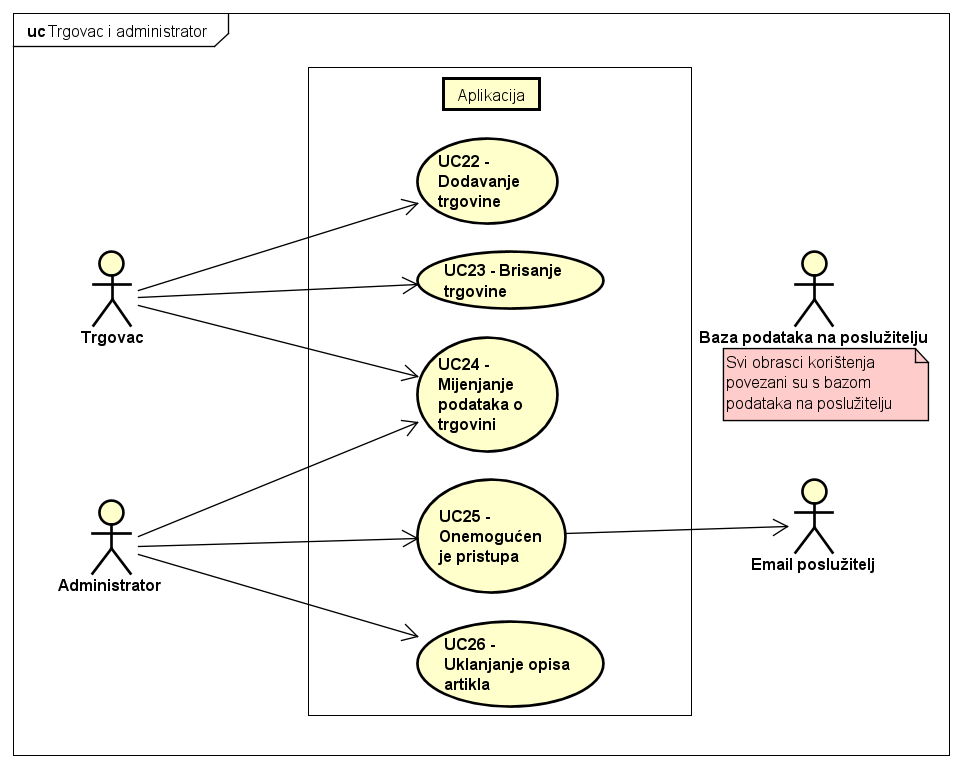
\includegraphics[width=.9\linewidth]{dijagrami/uc_trg_i_admin.png}
		            \label{fig:uc_trg_i_admin}
	                \end{center}
	            \end{figure}
	        
				\eject		
				
			\subsection{Sekvencijski dijagrami}
				
				\subsubsection{Obrazac uporabe UC7 - Dodavanje artikla na popis pretragom}
				    Korisnik pošalje traženo ime artikla. Poslužitelj iz baze podataka dohvaća barkodove i imena artikala sličnog imena. Prosljeđuje ih u listi korisniku. Ako lista nije prazna, korisnik odabire jedan od ponuđenih artikala i šalje poslužitelju njegov barkod i način izračuna cijene popisa, poslužitelj na temelju toga dohvati iz baze podataka informacije o artiklu i prosljeđuje ih cijenu korisniku. Korisnik ima sve potrebne informacije o stavci popisa i sprema ju u bazu podataka na uređaju.
	    \begin{figure}[H]
		    \centering
			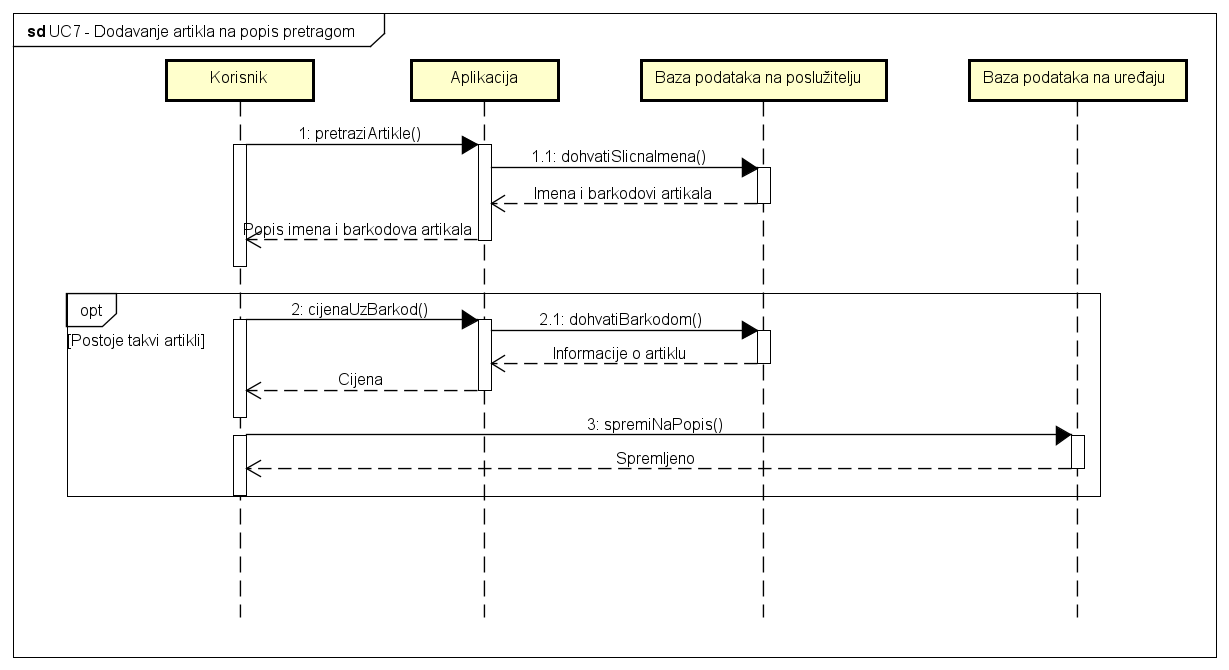
\includegraphics[width=0.9\linewidth]{dijagrami/sd_uc7.png}
			\caption{Sekvencijski dijagram za UC7}
			\label{fig:sd_uc7}
		\end{figure}
		
		
				\subsubsection{Obrazac uporabe UC13 - Prijava korisnika}
				    Ako se korisnik odlučio prijaviti Google računom, pošalje zahtjev za to poslužitelju koji provjerava njegove vjerodajnice zahtjevom prema Google poslužitelju. Ako su ispravne, u bazu podataka na poslužitelju sprema se token za korisnika i prijava je uspješna. Poslužitelj vraća rezultat prijave korisniku. \\
				    Ako se korisnik odlučio prijaviti email adresom i lozinkom, podatke za prijavu šalje na poslužitelj. Poslužitelj u bazi podataka provjerava jesu li ispravni. Ako jesu, poslužitelj sprema sjednički token u bazu podataka. na kraju poslužitelj vraća rezultat prijave korisniku. \\
				    Ako je korisnik odlučio zatražiti novu lozinku, šalje svoju email adresu poslužitelju. On provjerava u bazi podataka postoji li korisnik s tom email adresom. Ako postoji, generira privremenu lozinku, sprema ju u bazu podataka i šalje emailom korisniku preko email poslužitelja. Korisnik dobiva informaciju o tome je li lozinka poslana. \\
	    \begin{figure}[H]
		    \centering
			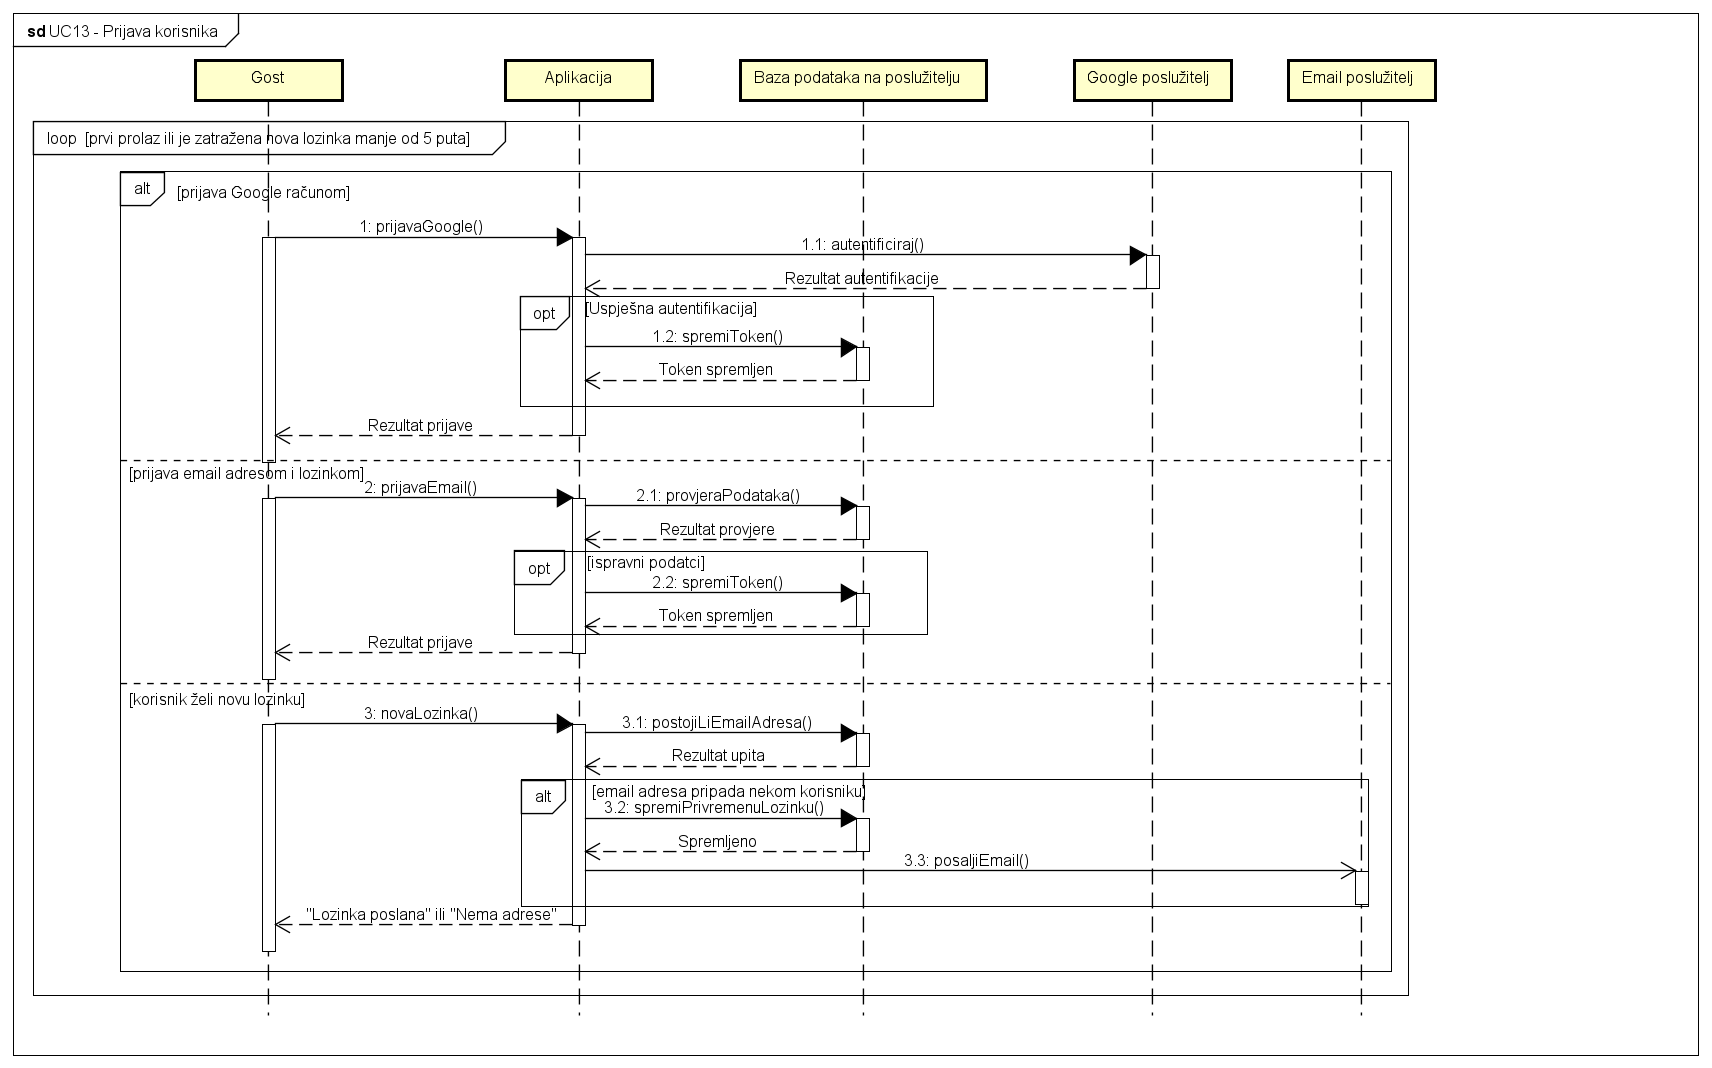
\includegraphics[width=1.0\linewidth]{dijagrami/sd_uc13.png}
			\caption{Sekvencijski dijagram za UC13}
			\label{fig:sd_uc13}
		\end{figure}
		
		
				\subsubsection{Obrazac uporabe UC17 - Izmjena informacija o artiklu}
				    Korisnik zatraži od poslužitelja informacije o artiklu. Korisnik dohvati informacije u bazi podataka i prosljeđuje ih korisniku. Ako korisnik zaključi da opis nije u redu, šalje zahtjev za smanjenjem broja glasova opisa. Poslužitelj ažurira broj glasova u bazi podataka i dohvati alternativne opise u bazi podataka koje zatim šalje korisniku. Ako se korisniku sviđa jedan od ponuđenih opisa, bira ga i tada se poslužitelju šalje zahtjev za povećanjem broja glasova opisa. Poslužitelj u bazi ažurira broj glasova i šalje korisniku povratnu informaciju. Ako se pak korisniku ne sviđa niti jedan od ponuđenih opisa, šalje svoj opis poslužitelju koji se sprema u bazu podataka i šalje zahtjev za smanjenjem broja glasova ponuđenih artikala. Poslužitelj ažurira broj glasova u bazi podataka i šalje povratnu informaciju korisniku.
	    \begin{figure}[H]
		    \centering
			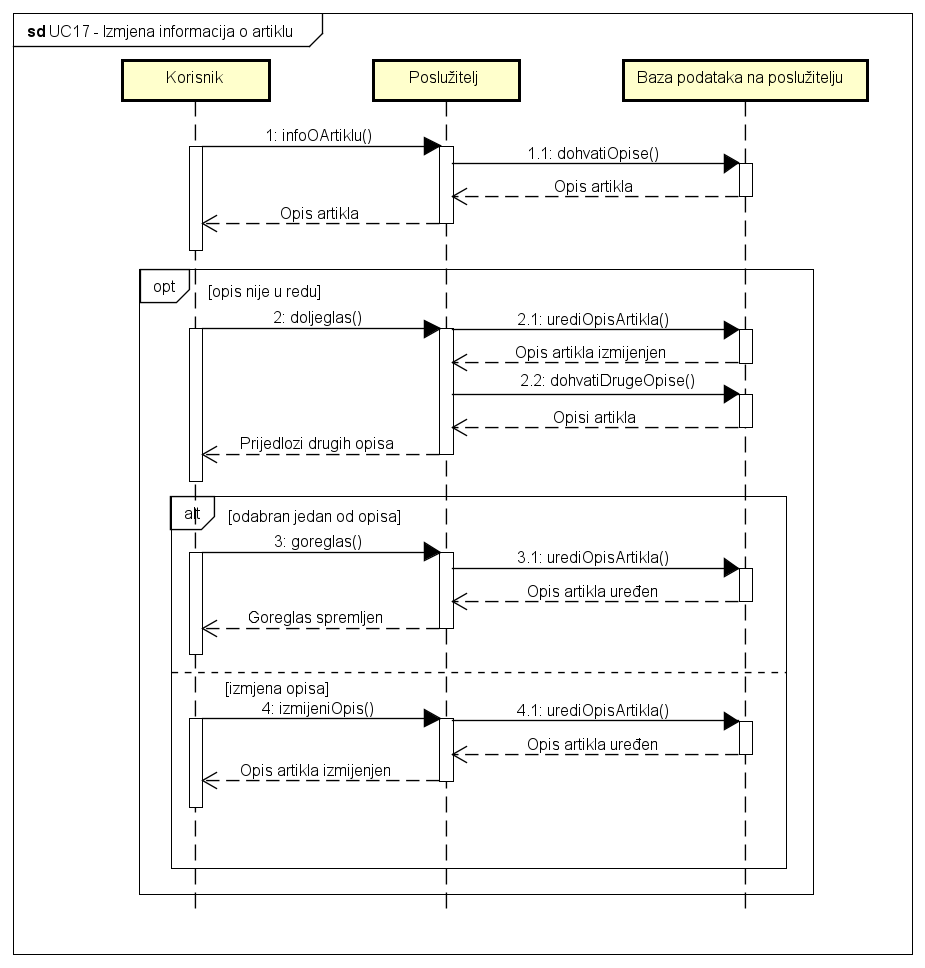
\includegraphics[width=1.0\linewidth]{dijagrami/sd_uc17.png}
			\caption{Sekvencijski dijagram za UC17}
			\label{fig:sd_uc17}
		\end{figure}
				\eject
	
		\section{Ostali zahtjevi}
        
        \begin{itemize}
            \item Aplikacija mora podržavati istovremeni rad 1000 korisnika
            \item Baza podataka mora odgovoriti na upit unutar pet sekundi
            \item Baza podataka mora podržavati unos 100 000 opisa artikala
            \item Baza podataka mora biti zaštićena od SQL injekcija
            \item Baza podataka mora biti otporna na napade duginom tablicom (rainbow table attack) dodavanjem predmetka lozinci
            \item Baza podataka mora lozinke raspršiti (hashing) pomoću funkcije SHA-256
            \item Pretpostavljena valuta sustava je HRK
            \item Korisničko sučelje mora podržavati hrvatski jezik i dijakritičke znakove
            \item Korisničko sučelje mora biti intuitivno
            \item Korisničko sučelje mora minimizirati broj koraka potrebnih da se učini neka akcija
            \item Neispravno korištenje korisničkog sučelja ne smije ugroziti rad sustava
            \item Aplikaciju mora biti moguće pokrenuti na Android uređajima inačice 5.0 naviše
        \end{itemize}
		 
			 %\textit{Nefunkcionalni zahtjevi i zahtjevi domene primjene dopunjuju funkcionalne zahtjeve. Oni opisuju \textbf{kako se sustav treba ponašati} i koja \textbf{ograničenja} treba poštivati (performanse, korisničko iskustvo, pouzdanost, standardi kvalitete, sigurnost...). Primjeri takvih zahtjeva u Vašem projektu mogu biti: podržani jezici korisničkog sučelja, vrijeme odziva, najveći mogući podržani broj korisnika, podržane web/mobilne platforme, razina zaštite (protokoli komunikacije, kriptiranje...)... Svaki takav zahtjev potrebno je navesti u jednoj ili dvije rečenice.}
			 
			 
			 
	
